\chapter{Implementación del controlador.}
% ----------------------

\label{C:Implementación del algoritmo de control}
\section{Implementación del Algoritmo de Control}
El desarrollo presentado en la sección  [\ref{C:Formas de control}] es fundamental para comprender las bases teóricas de las ecuaciones y estrategias que permiten calcular y determinar la acción de control adecuada, con el fin de lograr la mejor respuesta posible en la salida del sistema. Sin embargo, al llevar este algoritmo a una implementación real, es común encontrar variaciones de diseño debido a las condiciones no ideales de los componentes físicos, que difieren de sus contrapartes simuladas en software. En esta sección, se detallan los cambios necesarios para lograr un resultado funcional en la fuente de alimentación tras las pruebas realizadas con el primer prototipo, lo que condujo al diseño final.\par

\subsection{Condiciones de Funcionamiento}
Uno de los aspectos clave en el diseño de la fuente es la necesidad de garantizar que la magnitud de salida se mantenga estable a lo largo del tiempo, independientemente de las condiciones de carga. En este contexto, se identifican dos escenarios típicos: cuando hay una \textbf{carga conectada} a la salida y \textbf{cuando no la hay}. \par
Existe una diferencia notable entre ambos escenarios, ya que influyen directamente en el modo en que se disipa la energía almacenada en el capacitor de salida. Cuando hay una carga conectada, el capacitor se descarga más rápidamente, ya que la carga facilita la disipación de la energía, lo que significa desde el punto de vista del análisis de circuitos, un mayor amortiguamiento. En cambio, en condiciones de circuito abierto, el capacitor se descarga de manera más lenta debido a que la resistencia en paralelo $R_{16}$ de la figura \ref{F:Circuito_Actuador} está diseñada específicamente para permitir una descarga gradual cuando la fuente de alimentación se desconecta, lo que significa un menor amortiguamiento y por ende producir situaciones de inestabilidad o condiciones anormales de funcionamiento. Como resultado, en una transición de funcionamiento, la corriente que circulaba previamente hacia la carga puede terminar acumulándose en el capacitor de salida, incrementando su voltaje muy rápidamente. \par

\subsection{Rangos de Funcionamiento}
Otro aspecto fundamental a considerar es la necesidad de garantizar una respuesta transitoria rápida para cualquier valor de tensión y corriente de salida seleccionado. Dado que el comportamiento del sistema no es lineal en toda su gama de operación, el desempeño del algoritmo de control varía según la referencia de tensión establecida. Por ejemplo, la respuesta no es la misma al ajustar una referencia de 5V que al configurar una de 30V. Por esta razón, es necesario ajustar las constantes del control PID de manera específica para múltiples rangos de acuerdo al nivel configurado en la referencia, esto con el fin de optimizar el rendimiento y garantizar una acción de control más precisa en cada caso.\par

\subsection{Determinación de Escenarios}
El algoritmo de control implementado en la fuente de alimentación emplea un conjunto de criterios específicos para identificar si hay una carga conectada o si el circuito está en condición de vacío o carga reducida. El principal criterio se basa en la medición de los valores de corriente en la salida de la fuente. Si la corriente es cercana a cero, el algoritmo asume que el circuito está sin carga, interpretándose esta condición como un estado de vacío o condición de carga reducida. En cambio, si se detecta una corriente significativa, se infiere la presencia de una carga cuya magnitud es significativa dentro del rango de operación especificado. \par
Otro parámetro crucial para distinguir los escenarios es el comportamiento de la tensión una vez que se ha alcanzado su punto de estabilización. Un incremento brusco en el valor de la tensión sugiere la desconexión súbita de una carga, mientras que una disminución de la tensión de salida indica una perturbación en el sistema o la conexión de una carga adicional en paralelo. Estos cambios en la tensión permiten al algoritmo identificar la transición entre diferentes estados operativos.\par
Con base en estos criterios, el sistema evalúa la situación actual de la fuente y ajusta las constantes del controlador en el algoritmo para optimizar su respuesta ante las distintas condiciones de carga.\par

\section{Estrategia Empleada en el Algoritmo}
La combinación de diversas condiciones de carga y amplios rangos de funcionamiento llevó al desarrollo de un mapeo detallado de las zonas de mayor interés en el espectro de la fuente. En la Figura \ref{F:mapeo_cuadrantes}, se presenta un esquema de mapeo que divide las secciones en cuadrantes, cuyo objetivo es definir los valores de las constantes del controlador en función de las magnitudes registradas en cada momento. Para cada condición de operación, se asignan tres constantes al lazo de corriente y tres constantes adicionales al lazo de tensión, con una separación de 10 V entre ellas, abarcando un rango de 0 a 30 V. Esta estrategia permite lograr una respuesta transitoria más precisa y adecuada a los valores deseados en cada situación. \par

La implementación de esta estrategia responde a la complejidad inherente al comportamiento de la fuente, haciendo que la misma no pueda funcionar correctamente con un único diseño de control para todas las posibles variaciones de tensiones y corrientes dentro del rango especificado. Aplicar este enfoque asegura que la fuente se adapte dinámicamente a las distintas condiciones operativas, logrando así un funcionamiento estable y con tiempos aceptables de respuesta en diversos escenarios. Aunque la incorporación de más cuadrantes podría mejorar aún más el control, esto implicaría un mayor consumo de memoria en el procesador, ya que aumentaría la cantidad de valores flotantes necesarios. Tras realizar pruebas exhaustivas, se concluyó que el uso de seis zonas proporciona resultados satisfactorios en términos de eficiencia y precisión.\par


\begin{figure}[H]
    \centering
    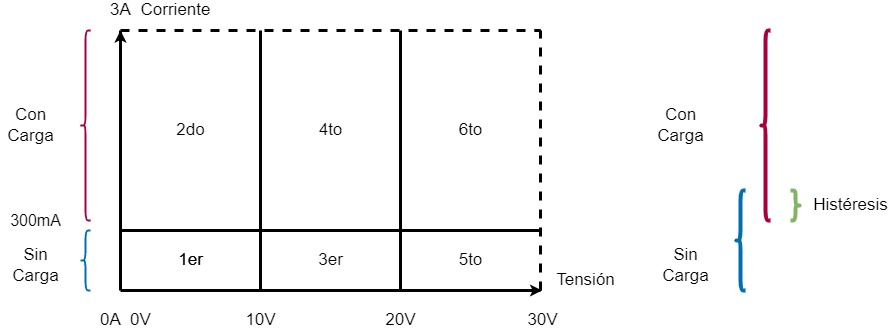
\includegraphics[width=1\textwidth]{./imagenes/matriz.jpg}
    \caption{Mapeo del rango de funcionamiento de la fuente.}
    \label{F:mapeo_cuadrantes}
\end{figure}\par

Un desafío de esta aproximación surge al acercarse a las zonas de transición entre las constantes del controlador, donde se produce un transitorio problemático en el cual el sistema podría perder estabilidad al cambiar de cuadrante. Para mitigar este inconveniente y asegurar que el controlador permanezca en el nuevo estado deseado, se desarrolló una ventana de histéresis como se ve en la parte derecha de la Figura \ref{F:mapeo_cuadrantes}. Esta ventana garantiza que la transición se complete de manera correcta, manteniendo la estabilidad del sistema en todo momento.\par


\subsection{Soft Reset}
Para evitar la confusión en el manejo de variables de control almacenadas en la memoria del dispositivo durante el funcionamiento, es fundamental mencionar la implementación de un \textit{soft reset} en el algoritmo de control. Este reinicio se encarga de restablecer todas las variables esenciales, como el error acumulado y el componente integrador, evitando que los valores previos influyan negativamente en el comportamiento del sistema cuando se pasa a un nuevo estado. El \textit{soft reset} permite que el sistema vuelva a un punto de referencia estable, similar al estado de reposo, garantizando así una respuesta controlada y óptima frente a nuevas condiciones de operación de la fuente, y previniendo posibles comportamientos indeseados como lo puede ser el aumento desmedido de la acción de control.\par


\subsection{Protección ante sobretensiones y falso contacto}
En sistemas electrónicos, es común que las cargas puedan tolerar valores de alimentación ligeramente inferiores al nominal durante unos pocos milisegundos hasta que la tensión se estabiliza. Sin embargo, esta tolerancia no se extiende a las sobretensiones, ya que incluso una sobretensión breve puede ser suficiente para dañar los componentes electrónicos de una carga. Por ello, la fuente de alimentación implementa un mecanismo de protección contra sobretensiones que desconecta de inmediato el relé de salida al detectar un valor de tensión superior al límite permitido. \par

Una vez eliminada la sobretensión y estabilizada la tensión de salida dentro de los límites predefinidos durante un tiempo determinado, el relé de salida se reactiva, permitiendo el acoplamiento seguro de la carga. Esta función es especialmente útil en casos de falso contacto, que pueden generar picos de tensión y perturbaciones en la salida de la fuente. Así, se proporciona una protección adicional a la carga, asegurando su integridad ante escenarios potencialmente dañinos. \par

Este mecanismo de protección no solo evita daños permanentes en los dispositivos conectados, sino que también garantiza una mayor durabilidad y fiabilidad del sistema en su conjunto, al reducir los riesgos asociados con fluctuaciones de tensión imprevistas. \par
